\question{Ширина спектральной линии излучения. Однородное и неоднородное 
уширения линий.}

Ширина линии в спектре излучения зависит от множества причин: \\
1) связанные с конечным временем жизни частицы в возбужденном состоянии
\[
\begin{array}{c}
  \D E \D\tau \geq \hbar = \frac{h}{2\pi}, \quad \D E \geq \cfrac{h}{2\pi\D\tau} \\ 
  \tau_0 = \D\tau, \quad E = h\nu_0, \quad \D E = h\D\nu_0 \\
  h\D\nu_0 = \cfrac{h}{2\pi\tau_0}, \quad \D\nu_0 = \cfrac{1}{2\pi\tau_0}
\end{array}
\]
где \( \D\nu_0 \) -- уширение линии \\
2) в следствии хаотического движения и столкновения частиц время жизни в 
возбужденном состоянии может сокращаться относительно рассматриваемого 
\( \tau_0 \), что приведёт также к уширению линии
\[ 
  \D\nu_\text{ст} = \frac{1}{2\pi\tau_\text{ст}} 
    \text{ -- столкновительное уширение} 
\]
\[
  \tau_\text{ст} = \frac{1}{n<\sigma_\text{ст}\cdot v>} = 
  \left\{ \begin{array}{c}
    n \text{ -- концентрация} \\
    \sigma_\text{ст} \text{ -- столкновительное сечение} \\
    v \text{ -- скорость}
  \end{array} \right\} = \frac{1}{n\sigma_\text{ст}v}
\]

Уширение линии связано с этими причинами [1,2] -- однородное уширение. 
Поскольку эти процессы вероятностны, то они описывают распределение плотности 
вероятности так называемый форм-фактор в данном случае Лоренцев контур.

\begin{figure}[h]
  \center
    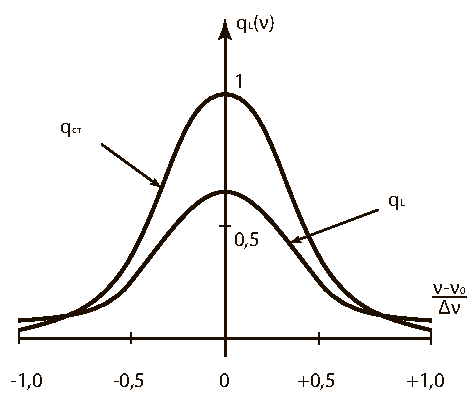
\includegraphics[width=.47\textwidth]{05_01}
\end{figure}
\[
\begin{array}{c}
  \nu_0 = \cfrac{\D E}{h} \\
  q_L(\nu) = \frac{\D\nu_L}{2\pi
    \left[ (\nu-\nu_0)^2 + \left( \frac{\D\nu_L}{2} \right)^2\right]} \\
  \D\nu_L = \D\nu_0 + \D\nu_\text{ст} \\
\end{array}
\]
\( \D\nu_L \) -- полная ширина линии на половине высоты.

Уширенными являются все энергетические уровни частицы, за исключением основного 
(время жизни основного уровня бесконечно и \( \D\nu = 0 \)). Уширение линии 
связано с конечным временем жизни в возбужденном состоянии называется 
однородным. \\
3) конечное время жизни частицы не является единственной причиной уширения

В следствии движения частицы относительно приёмника излучения наблюдается 
изменение частоты обусловленное эффектом Доплера.
\[
  \D\nu_D = \nu_0 \frac{\vec{v}}{c}\cos\phi
\]

Так как излучающие частицы движутся с различными скоростями и в различных 
направлениях, то частотные сдвиги излучаемых ими линий различны. Поэтому даже 
в случае отсутствия столкновений неподвижный спектральный прибор будет 
регистрировать множество естественно уширенных линий, различно смещенных 
относительно частоты \( \nu_0 \). Это так называемое \emph{доплеровское 
уширение}, которое является продуктом деятельности коллектива частиц, такое 
уширение -- неоднородное.